\section{Geometric Primal-Dual Framework}\label{sec:geo-primal-dual}

Let $\sigma$ be an input to the $k$-SP problem, where the distance between two locations $a$ and $b$ is given by $\distance{a}{b}=\|a-b\|_p$. In this section, we introduce a primal-dual framework based on hierarchical partitioning to compute a minimum-cost $(n-k)$-matching in $\mcG_\sigma=(A\cup B, E\subset A\times B)$. We begin by describing the hierarchical partitioning scheme.

%be the bipartite graph constructed in Section~\ref{sec:introduction} for the $k$-SP instance under the $\ell_p$ norm for a parameter $p\ge 1$, i.e., $\distance{a}{b}=\|a-b\|_p$ for all $(a,b)\in E$, in this section, we present a partitioning-based primal-dual framework for computing an optimal $(n-k)$-matching on $\mcG_\sigma$. We begin by describing a hierarchical partitioning scheme.


\subsection{Hierarchical Partitioning}\label{sec:hierarchical}
Using $\lambda:=9n^{-1/5}$, we construct a hierarchical partitioning $\mcH$ recursively. Each node of $\mcH$ is an axis-parallel rectangle, referred to as a \emph{cell}. The root node, $\cell^*:=[-3n, 3n]^2$, contains all points in $A\cup B$. For each node $\cell$, let $A_\cell$ and $B_\cell$ be the points of $A$ and $B$ inside $\cell$ and let $n_{\cell}=|A_\cell \cup B_{\cell}|$. If $n_{\cell}\le2$ (i.e., $\cell$ is empty or contains the entry and exit gates of a single request), then $\cell$ is marked as a leaf node. Otherwise, we partition $\cell$ into two smaller rectangles as follows. Let $\ell_\cell$ be the larger of the length and width of rectangle $\cell$. Without loss of generality, assume that $\ell_\cell$ is the width of $\cell$ and let $x_{\min}$ be the $x$-coordinate of the bottom-left corner of $\cell$.   For any value $\hat{x}\in [x_{\min}+\frac{\ell_\cell}{3}, x_{\min}+\frac{2\ell_\cell}{3}]$, define $\Lambda(\hat{x}):=\{u\in A_\cell\cup B_\cell: |u_x-\hat{x}|\le \ell_\cell\lambda\}$; here, $u_x$ denotes the $x$ coordinate of the point $u$. Let $x^*:=\arg\min_{\hat{x}\in [x_{\min}+\frac{\ell_\cell}{3}, x_{\min}+\frac{2\ell_\cell}{3}]}|\Lambda(\hat{x})|$. 
We partition $\cell$ into two smaller rectangles by using a vertical line defined by $x=x^*$ and add them as the children of $\cell$ to $\mcH$. We refer to the segment partitioning $\cell$ into its two children as its \emph{divider} and denote it by $\divider\cell$. See Figure~\ref{fig:hierarchical}. For any cell $\cell$, the four sides of its rectangle are defined by the dividers of its ancestor or the boundaries of the root square.
This completes the construction of $\mcH$. Note that the height of the tree is $O(\log n\Delta)$. A simple sweep-line algorithm can compute $x^*$ in $O(n_\cell\log n_\cell)$ time. Using this procedure, we construct $\mcH$ in $\tilde{O}(n \log (n\Delta))$ time.
\begin{figure}
    \centering
    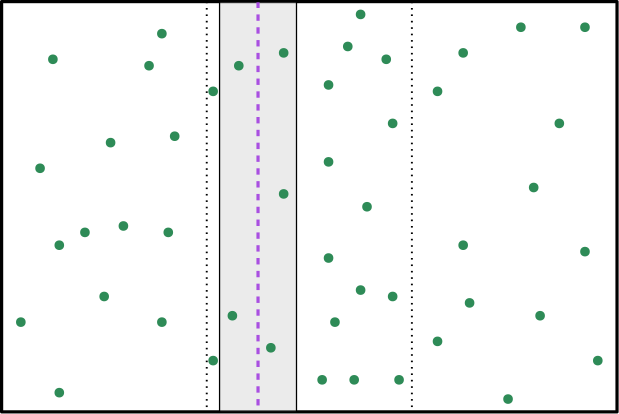
\includegraphics[width=0.6\linewidth]{figures/grid2.png}
    
    \caption{We Partition a rectangle into two children by picking a divider (the purple dashed vertical line) with the minimum number of points close to it (gray shaded area) within the middle-third of its longer side (the part between the two vertical dotted lines).}
    \label{fig:hierarchical}
\end{figure}


\begin{restatable}{lemma}{margin}\label{lemma:margin}
    For each cell $\cell$ of $\mcH$, the ratio of the largest to the smallest side of $\cell$ is at most $3$. Furthermore, the number of points of $A_\cell\cup B_\cell$ with a distance smaller than $\ell_\cell\lambda$ to the divider $\divider\cell$ is $O(n_\cell\lambda)$.
\end{restatable}


Recollect that a matching $M$ in $\mcG_\sigma$ is a subset of vertex-disjoint edges. We refer to a point $b\in B$ as \emph{unmatched} in $M$ if it does not have an edge of $M$ incident on it and \emph{matched} otherwise. 
The following structural property of the $k$-SP problem will be critical in bounding the efficiency of our algorithm.

\begin{restatable}{lemma}{geometricAnalysis}\label{lemma:geometric-matching}
    For any cell $\cell$ of $\mcH$, there exists a matching $M'$ between $A_\cell\cup B_\cell$ that matches all except $O(n_\cell^{4/5})$ points of $B_\cell$ and has a cost $O(\ell_\cell n_\cell^{3/5})$.
\end{restatable}
\begin{proof}
We place a grid $G$ with cell-side-length $\ell_\cell n_\cell^{-2/5}$ inside $\cell$. For each square $\xi$ of $G$, let $\requests_\xi$ denote the subset of requests that lie inside $\xi$, and define $M_\xi$ to be the bipartite matching that corresponds to a single server serving the requests of $\requests_\xi$. Define $M':=\bigcup_{\xi\in G}M_\xi$. See Figure~\ref{fig:extended_matching}(left). 
\end{proof}

\begin{figure}
    \centering
    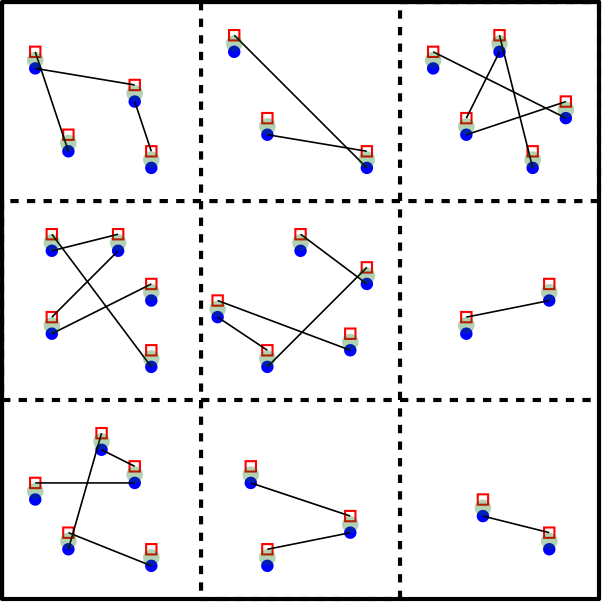
\includegraphics[width=0.4\linewidth]{figures/geo.png}\hspace{2em}
    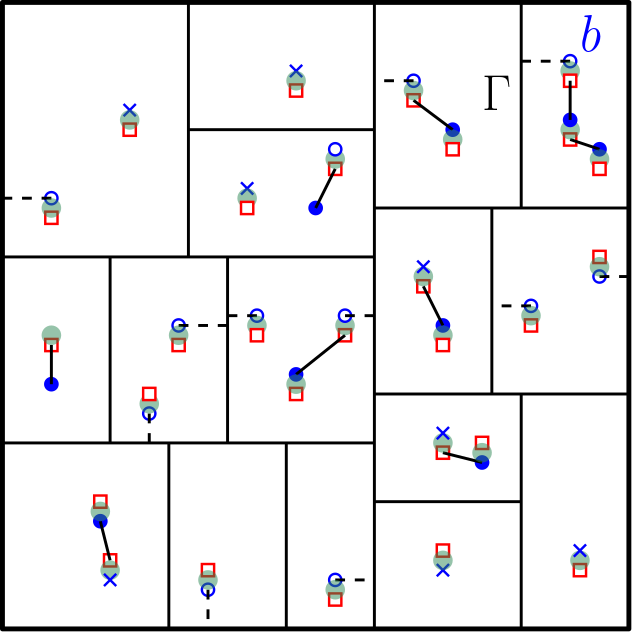
\includegraphics[width=0.4\linewidth]{figures/extended3.png}
    \caption{(left) The low-cost high-cardinality matching constructed inside a cell $\cell$ of $\mcH$, and (right) a $\mcC$-extended $20$-matching with $9$ matched points (blue discs), $11$ boundary-matched points (blue circles), and $8$ free points (blue crosses). The matching cost is the total length of the solid and dashed lines. The boundary-matched point $b$ is matched to the boundary $\Gamma$.}
    \label{fig:extended_matching}
\end{figure}



\subsection{Extended Bipartite Matching}\label{sec:primal}
Suppose we are given a subset $\mcC$ of cells from $\mcH$ that partitions $\cell^*$, i.e., the cells of $\mcC$ are interior disjoint and these cells cover the root square $\cell^*$. Let $\distance{u}{\cell}$ denote the shortest distance from $u$ to the boundaries of the cell $\cell$. For any point $u$ inside $\cell^*$, let $\cell_u$ be the cell of $\mcC$ that contains $u$. We define $\distance{b}{\mcC} = \distance{b}{\cell_b}$. We extend the definition of matching to allow points in $B$ to match to the boundaries of cells in $\mcC$. A \emph{$\mcC$-extended matching} consists of a matching $M$ as well as a subset $B^\mcC$ of points of $B$ that are unmatched in $M$ but instead matched to the boundaries of the cells of $\mcC$ that contain them. See Figure~\ref{fig:extended_matching}(right). The cost of a $\mcC$-extended matching $M^\mcC$ is
\begin{equation}
    w_\mcC(M^\mcC) := \sum_{(a,b)\in M} \distance{a}{b} + \sum_{b \in B^{\mcC}} \distance{b}{\mcC}.
\end{equation}

We refer to all points of $B^{\mcC}$ as \emph{boundary-matched}. All points of $B$ that are neither matched in $M$ nor boundary-matched are considered \emph{free}. All points of $A$ that are not matched in $M$ are also considered free. The size of $M^{\mcC}$ is equal to $|M|+|B^{\mcC}|$. When $\mcC$ is clear from the context, we refer to $M^{\mcC}$ as an extended matching. An extended matching $M^{\mcC}$ of size $t$ with the minimum cost is called a \emph{minimum-cost $\mcC$-extended $t$-matching}.





Consider the partitioning $\mcC^*=\{\cell^*\}$, where $\cell^*$ is the root cell of $\mcH$. Using the fact that the input points are far from the boundaries of $\cell^*$, we show in Lemma~\ref{lemma:root-inactive} below that any minimum-cost $\mcC^*$-extended matching $M^{\mcC^*}$ of size $t$ is also a minimum-cost $t$-matching, i.e., no point of $B$ is boundary-matched in $M^{\mcC^*}$. 
\begin{restatable}{lemma}{rootinactive}\label{lemma:root-inactive}
    Suppose $\mcC^*=\{\cell^*\}$, where $\cell^*$ is the root cell of $\mcH$. Let $M^{\mcC^*}=(M, B^{\mcC^*})$ be a minimum-cost extended $t$-matching on $\mcG_\sigma$, for $t<n$. Then, the matching $M$ is a minimum-cost $t$-matching.
\end{restatable}


Let $M^\mcC=(M, B^\mcC)$ denote a $\mcC$-extended matching.
Any path $P$ on the graph $\mcG_\sigma$ whose edges alternate between matching and non-matching edges in $M$ is called an \emph{alternating path}. 
An alternating path $P$ is called an \emph{augmenting path} if $P$ starts from a free point $b\in B$ and ends with either (i) a free point $a\in A$, or (ii) a point $b'\in B$.  We \emph{augment} the extended matching $M^{\mcC}$ along an augmenting path $P$ by updating its matching $M\leftarrow M\oplus P$ and for case (ii), we match $b'$ to the boundary and update $B^\mcC$ to include $b'$. The \emph{net-cost} of $P$ in case (i) is $\phi(P):=\sum_{(a,b)\in P\setminus M}\distance{a}{b} - \sum_{(a,b)\in P\cap M}\distance{a}{b}$, and 
in case (ii) is \[\phi(P):=\distance{b'}{\mcC} + \sum_{(a,b)\in P\setminus M}\distance{a}{b} - \sum_{(a,b)\in P\cap M}\distance{a}{b}.\] 


From Lemma~\ref{lemma:root-inactive}, given a sequence $\sigma$ of $n$ requests in the unit square, one can compute an optimal solution to the $k$-SP problem on $\sigma$ by computing a minimum-cost $\mcC^*$-extended $(n-k)$-matching on $\mcG_\sigma$. Given a partitioning $\mcC$, to compute a minimum-cost $\mcC$-extended $(n-k)$-matching, similar to the Hungarian algorithm, one can start from an empty extended matching $M^\mcC$ and iteratively augment $M^\mcC$ along a minimum net-cost augmenting path. In the next section, we present a primal-dual framework that our algorithm uses to efficiently compute minimum net-cost augmenting paths.




\subsection{A Constrained Dual Formulation for Extended Matchings}\label{sec:dual}
Suppose $\mcC$ is a set of cells of $\mcH$ partitioning the root cell $\cell^*$. Consider a $\mcC$-extended matching $M^\mcC=(M, B^\mcC)$ on $\mcG_\sigma$ along with a set of non-negative dual weights $y:A\cup B\rightarrow \mbR_{\ge0}$. Let $A_F$ be the set of free points of $A$ with respect to $M^\mcC$. We say that $M^{\mcC}, y(\cdot)$ is \emph{feasible} if,
\begin{align}
    y(b) - y(a) &\le \distance{a}{b},&  \quad \forall(a,b)&\in E,\label{eq:dualfeasibility-non-matching-time}\\
    y(b) - y(a) &= \distance{a}{b},& \quad \forall(a,b)&\in M,\label{eq:dualfeasibility-matching-time}\\
%\end{align}
%and for any cell $\cell\in\mcC$, 
%\begin{align}
    y(b) &\le \distance{b}{\mcC},&  \quad \forall b&\in B,\label{eq:dualfeasibility-b}\\
    y(b) &= \distance{b}{\mcC},&  \quad \forall b&\in B^\mcC,\label{eq:dualfeasibility-b-admissible}\\
    y(a) &= 0,& \quad \forall a&\in A_F.\label{eq:dualfeasibility-a-free}
\end{align}

For any  edge $(a,b)\in E$, the \emph{slack} of $(a,b)$ is defined as $s(a,b):=\distance{a}{b} - y(b) + y(a)$. The edge $(a,b)$ is \emph{admissible} if $s(a,b)=0$. For any point $b\in B$, the slack of $b$ is defined as $s(b):=\distance{b}{\mcC} - y(b)$. For any feasible extended matching $M^{\mcC}, y(\cdot)$, the slack of every edge as well as every point $b \in B$ is non-negative.
Recall that an augmenting path $P$ starts at a free point $b\in B$ and ends at (i) a free point $a\in A$ or (ii) a point $b'\in B$. The path $P$ is \emph{admissible} if all edges of $P$ are admissible and in case (ii), the slack of the end-point $b'$ is $s(b')=0$.
The following properties of extended feasible matchings are critical in the design of an efficient and correct algorithm.


\begin{restatable}{lemma}{netcost}\label{lemma:augpath}
Given a feasible $\mcC$-extended $t$-matching $M^{\mcC} = (M, B^{\mcC})$ and a set of non-negative dual weights $y(\cdot)$ on $A\cup B$, let $P$ be a minimum net-cost augmenting path with respect to $M^{\mcC}$. Let, for any $\cell \in \mcC$, $y_\cell=\max_{b' \in B_{\cell}} y(b')$.
Then, 
\begin{itemize}
\item[(a)] all points of $P$ lie inside a single cell of $\mcC$, and
\item[(b)] if, for every cell $\cell \in \mcC$, $y_\cell \le \phi(P)$ and for all free points $b\in B_\cell$, $y(b) = y_\cell$, then $M^\mcC$ is a minimum-cost extended $t$-matching.
\end{itemize}
\end{restatable}

\vspace{1em}
The property described in Lemma~\ref{lemma:augpath}(a) is important for the design of an efficient algorithm. Unlike the Hungarian algorithm, which searches the entire graph for the minimum net-cost augmenting path, our algorithm can find the minimum net-cost augmenting path by searching for the cheapest augmenting path inside each cell $\cell \in\mcC$ and then taking the smallest among them. Thus, we can replace a global search with a search inside each cell of $\mcC$.
The property in Lemma~\ref{lemma:augpath}(b) is important for the design of a correct algorithm since it provides conditions under which an extended matching is a minimum-cost extended matching. Our algorithm is designed to maintain these conditions as invariants during its execution.  
Lemma~\ref{lemma:fresh_duals} provides a method to update the dual weights, which will be essential during the process of merging cells.


\begin{restatable}{lemma}{updateDuals}\label{lemma:fresh_duals}
        Suppose $M^\mcC, y(\cdot)$ is a feasible $\mcC$-extended matching and $P$ is a minimum net-cost augmenting path. For any cell $\cell\in\mcC$, define $y_\cell=\max_{b' \in B_{\cell}} y(b')$, and suppose $y_\cell\le \phi(P)$ and $y(b_f)=y_\cell$ for all free points $b_f\in B_\cell$. Then, one can update the dual weights in $\tilde{O}(n_\cell\Phi(n_\cell))$ time such that $M^\mcC, y(\cdot)$ remains feasible, $y(b)\le \phi(P)$ for all $b\in B_\cell$, and $y(b_f)=\phi(P)$ for all free points $b_f\in B_\cell$.
\end{restatable}

\vspace{0.5em}
The next lemma provides critical properties that allow for correctly and efficiently merging cells in $\mcC$. 


\begin{restatable}{lemma}{combination}\label{lemma:combination}
    For a cell $\cell$ of $\mcH$, suppose $\cell'$ and $\cell''$ denote its two children, and let $\mcC$ denote a partitioning containing $\cell'$ and $\cell''$. Let $\mcC'=\mcC\cup\{\cell\}\setminus\{\cell',\cell''\}$. Given a feasible $\mcC$-extended matching $(M, B^\mcC), y(\cdot)$, let $B_\cell^\mcC\subseteq B^\mcC$ denote the subset of boundary-matched points that are matched to the divider $\Gamma_\cell$ of $\cell$. Then,
    \begin{itemize}
        \item[(a)] the $\mcC'$-extended matching $(M, B^\mcC\setminus B_\cell^\mcC), y(\cdot)$ is also feasible, and,
        \item[(b)]  $|B_\cell^\mcC|=O(n^{4/5})$.
    \end{itemize}
\end{restatable}

\vspace{1em}

From Lemma~\ref{lemma:combination}(a), erasing a divider  does not cause the feasibility conditions to be violated. The proof of Lemma~\ref{lemma:combination}(a) relies on the fact that when we erase the divider of a cell in $\mcC$, the RHS of~\eqref{eq:dualfeasibility-b} will only increase and so it is not violated. Despite preserving the feasibility conditions, erasing the boundary may result in the violation of Lemma~\ref{lemma:augpath}(b), i.e., the matching may no longer be a minimum-cost extended matching. 
%This is because the condition of Lemma~\ref{lemma:augpath}(b) may be violated.
In our algorithm in Section~\ref{sec:k-seq}, we describe a process to adjust the matching $M^\mcC$ and dual weights $y(\cdot)$ and obtain a minimum-cost extended matching. 


\myparagraph{Residual Graph.}
Similar to the Hungarian algorithm, we define a residual graph that assists in finding the minimum net-cost augmenting path. Consider a feasible $\mcC$-extended matching $M^{\mcC}=(M,B^{\mcC})$ along with a set of dual weights $y(\cdot)$ on points of $A\cup B$. For each cell $\cell \in \mcC$, we define a residual graph $\mcG_{\cell}$. The vertex set of $\mcG_{\cell}$ is a source vertex $s$ and the points in $A_{\cell}\cup B_{\cell}$. For any edge $(a,b)\in E$ inside $\cell$, if $(a,b)$ is an edge in $M$ (resp. not an edge in $M$), there is an edge directed from $a$ to $b$ (resp. from $b$ to $a$) with a weight $s(a,b)$ in $\mcG_\cell$. Furthermore, there is an edge directed from $s$ to every free point $b\in B$ with a weight $y(b)$.
